\section{COCOMO analysis}
The COCOMO model allows to estimate the time effort required by the project. We use the version of this model called COCOMO II. It is based on a main formula:
\begin{equation}
PM = A * Size^{E} * \prod_{1<=i<=n}^{} EM_{i} 
\end{equation}

where:
\begin{itemize}
	\item \textbf{PM} stands for "Person-Months"
	\item \textbf{A}=2.94. It approximates a productivity constant in PM/KSLOC for the case where E = 1.0.
	\item \textbf{Size} is measured in KSLOC and is the result of the Function Points analysis.
	\item \textbf{E} is an aggregation of 5 \textbf{scale factors}:
	\begin{itemize}[label = {-}]
		\item \textbf{Precedentedness:} It is high if the project is similar to several previous projects
		\item \textbf{Development Flexibility:} It is high if there are no specific constraints to conform to pre-established     requirements and external interface specifications.
		\item \textbf{Architecture / Risk Resolution:}It is high if the project plan includes a good risk management plan, a clear definition of budget and schedule, with a focus on architectural definition
		\item \textbf{Team Cohesion:} It is high if all stakeholders are able to work in a team and share the same vision and commitment.
		\item \textbf{Process Maturity:} Refers to a well known method for assessing the maturity of a software organization, CMMI, that is a process level improvement training and appraisal program.
	\end{itemize}
	\begin{figure}[H] 
		\centering
		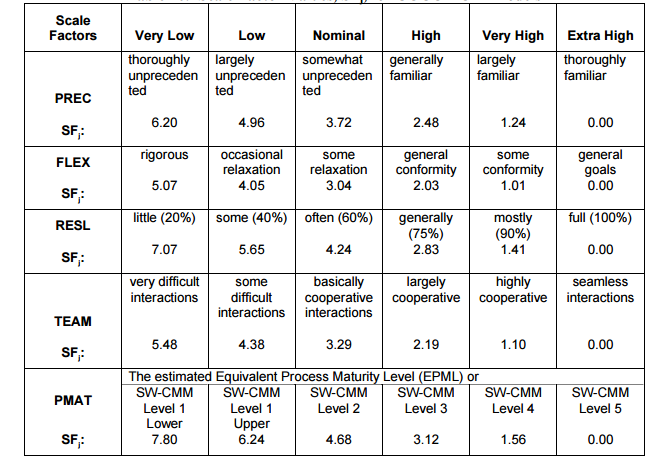
\includegraphics[scale = 0.7]{img/scaleFactors.png}
		\caption{Scale Factors}
	\end{figure}
	
	E is calculated with the formula:
	\begin{equation}
	E = B + 0.01 * \sum_{1<=j<=5}^{} SF_{j}
	\end{equation}
	where B=0.91
\end{itemize}


\subsection{Scale Factors}
\subsubsection{Precedentedness}
For our development team is the first project done in the field of Car Sharing involving electric cars and so the personnel has no previous knowledge about it. For this reason we consider the Precedentedness of our project \textbf{very low}.\\
\textbf{PREC=6.20}

\subsubsection{Development Flexibility}
As for pre-established requirements, the development team is provided with a lot of requirements about the application and the service to be considered. On the other hand, there is no constraint on external interfaces to be considered.
So, taking the average of the low flexibility for requirements and the high flexibility on external interfaces, the resulting Development Flexibility is \textbf{nominal}.\\
\textbf{FLEX=3.04}

\subsubsection{Architecture / Risk Resolution}
Considering that the people in charge of project planning are new to this job, but they are also very motivated and able to learn fast, we can consider that their work on the risk management plan and the definition of budget and schedule has a \textbf{nominal} rate, taking the average of the low experience and the personnel characteristics.\\
\textbf{RESL=4.24}

\subsubsection{Team Cohesion}
The group working on the project has newly been assembled, so its cohesion is in general unknown. Nevertheless, the people selected to join the group are all young, motivated, open-minded and suitable for group-works, so we can consider the Team Cohesion \textbf{nominal}, taking the average of high uncertainty and good skills of the personnel.\\
\textbf{TEAM=3.29}

\subsubsection{Process Maturity}
The maturity level of the project is \textbf{2}, for this reasons:

\begin{itemize}
	\item The processes of our project will be planned and executed according to specific and clear criteria. 
	\item The people that will work on the project have been selected among a wide list of candidates and only the one that have demonstrated to have the best skills have been chosen.
	\item We consider the resources provided by the customer and the ones already owned by the development team adequate.
	\item We have the purpose of involving in the processes all the stakeholders as much as possible, to have frequent feedbacks and suggestions on the works
	\item Having the purpose of receiving feedbacks, we will use them and other evaluations to check the adherence of the project to requirements.
	\item The development team is focused only on the PowerEnJoy project, so of course the processes are planned, documented, performed,monitored and controlled at the project level.
	\item Because the development team has no previous knowledge about the field of car sharing, it will have mainly a reactive behaviour, because it cannot predict problems that it doesn't know.  
\end{itemize}  
\textbf{PAMT=4.68}

\pagebreak
\subsection{Effort Multiplier}
\textbf{EM} stands for Effort Multiplier. Effort multipliers are derived from \textbf{Cost drivers}. The selection of these cost drivers depends on wh1ether the project regards a \textbf{Post-Architecture} system or a \textbf{Early Design} system. We are in the Early Design case, because we are extending an existing product and our system will be developed from scratch. So the cost drivers are:

\subsubsection{Personnel Capability}
Personnel Capability (PERS) is a combination of Analyst Capability(ACAP), Programmer Capability(PCAP) and Personnel Continuity cost driver of Post-Architecture.

			In our case we have little experience in the software analysis but this is balanced by good programming skills. The combination of ACAP and PCAP can be considered as \textbf{"Nominal"}
			
			\textbf{PERS=1.0}
\begin{figure}[H] 
	\centering
	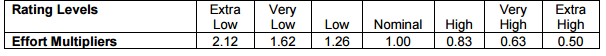
\includegraphics[scale = 0.6]{img/PERS.png}
	\caption{EMs of PERS}
\end{figure}
		

			
\subsubsection{Product Reliability and Complexity}
	Product Reliability and Complexity(RCPX) is a combination of Required Software Reliability(RELY), Data Base Size(DATA), Product Complexity(CPLX) and Documentation Match to Life-Cycle Need(DOCU) cost drivers of Post-Architecture. 
			\\
			The software reliability is very important because a failure of the system can potentially cause a huge financial loss.\\
			The DATA cost driver attempts to capture the effect large test data requirements have on product development. For this particular driver we don’t have enough information to do a reliable estimation so the value can be considered \textbf{"Nominal"}.\\
			We decided to assign the complexity of the system a value \textbf{"Very high"}
			
		
			\textbf{RCPX=1.33}

\begin{figure}[H] 
	\centering
	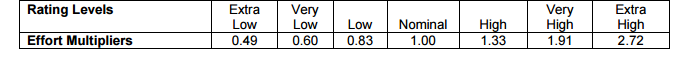
\includegraphics[scale = 0.6]{img/RCPX.png}
	\caption{EM of RCPX}
\end{figure}
	
		
\subsubsection{Developed for Reusability}		
			There are no requirement on Reusability so the value is considered \textbf{"Nominal"}
			
			\textbf{RUSE=1.0}
			
		\begin{figure}[H] 
			\centering
			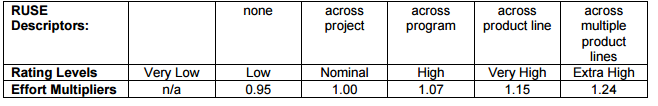
\includegraphics[scale = 0.6]{img/RUSE.png}
			\caption{EMs of RUSE}
		\end{figure}

\subsubsection{Platform Difficulty}		
Platform Difficulty (PDIF) is a combination of Execution Time Constraint(TIME), Main Storage Constraint(STOR) and Platform Volatility(PVOL) cost drivers of Post-Architecture. 
		\\
		The OnBoard device is real-time embedded product so the execution time is important, but on the rest of the system there are no particular constraint about the execution time. Same as before there are no requirements on Storage.
		Platform Volatility can be considered \textbf{"Very high"} because the system is composed of different part on different system (OnBoard Device, Application Logic on server, Client on smartphone or browser).
		\\
		\textbf{PDIF=1.29}
		
		\begin{figure}[H] 
			\centering
			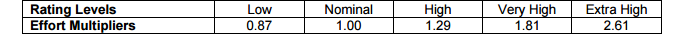
\includegraphics[scale = 0.6]{img/PDIF.png}
			\caption{EMs of PDIF}
		\end{figure}
	
\subsubsection{Personnel Experience}		
{Personnel Experience (PREX) is a combination of Application Experience(APEX), Platform Experience(PLEX), Language and Tool Experience(LTEX) cost drivers of Post-Architecture. 
			\\
			Because of the team inexperience the overall value is considered \textbf{"low" }
			\\
			\textbf{PREX=1.22}
		\begin{figure}[H] 
			\centering
			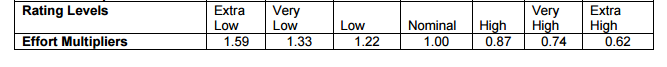
\includegraphics[scale = 0.6]{img/PREX.png}
			\caption{EMs of PREX}
		\end{figure}

\subsubsection{Facilities }		
Facilities (FCIL) is a combination of Use of Software Tools(TOOL) and Multisite Development(SITE) cost drivers of Post-Architecture. 
		\\
		Because of the entity and the life-cycle of the product development there are different system and tools that need to be integrated to develop the whole product so TOOL is considered \textbf{"Low"}.
		With all the new collaboration tools (Slack, github, Skype) the Multi-Site development driver is considered \textbf{"Nominal"}
		\\
		\textbf{FCIL=1.10}
		\begin{figure}[H] 
			\centering
			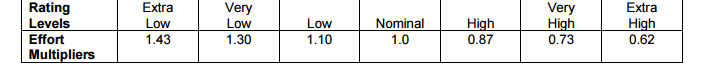
\includegraphics[scale = 0.6]{img/FCIL.png}
			\caption{EMs of FCIL}
		\end{figure}

\subsubsection{Required Development Schedule }		
	Required Development Schedule (SCED):
		\\
		Non accelerated Waterfall Developement Schedule so it's considered \textbf{"Nominal"}.
		\\
		\textbf{SCED=1.0}
		
		\begin{figure}[H] 
			\centering
			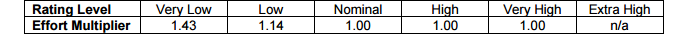
\includegraphics[scale = 0.6]{img/SCED.png}
			\caption{EMs of SCED}
		\end{figure}
	



\begin{table}[H]
	\centering
	\resizebox{\textwidth}{!}{%
		\begin{tabular}{lllllllll}
			\hline
			\textbf{Driver} & PERS & RCPX & RUSE & PDIF & PREX & FCIL & SCED & Product   \\ \hline
			\textbf{Value}  & 1.0  & 1.33 & 1.0  & 1.29 & 1.22 & 1.10 & 1.0  & 2.3024694 \\ \hline
		\end{tabular}%
	}
	\caption{EM Result Table}
\end{table}

\FloatBarrier

\subsection{Results} 
According to the Scale Factors and the Effort Multiplier

$$Effort = A * KLOC^{E} * EAF$$
$$A=2.94$$
$$EAF=\prod_{1<=i<=n}^{} EM_{i} \approx2.3$$
$$E=0.91+0.01*21.45$$
\\
Total effort result in persons months:
$$PM = 34.70$$

%1,33*1,29*1,22*1,1=2,3024694

\begin{equation}
Duration = 3.67 * (PM)^{(0.28+0.2 * (E - 0.91))}
\end{equation}



